\SourceLeaf{325}
dass das obige Criterium in so fern nicht ganz allgemein ist, als es stillschweigend voraussetzt, dass keiner der betreffenden Sinus $=0$ ist. Zur Vervollständigung müsste noch beigefügt werden:

1) ist \textls[120]{Einer} der drei Sinus $=0$, z.\,B. der erste, aber keiner der beiden andern, so fällt 0 mit 1 zusammen, wo natürlich für die Richtung 01 jeder beliebige Werth genommen werden kann.

2) Sind \textls[120]{zwei} $=0$, so wird von selbst auch der dritte $=0$ (weil die Summe der drei Winkel identisch $=0$ ist). In diesem Fall ist die \textsc{Pothenot}sche Aufgabe entweder unbestimmt oder physisch unmöglich; das zweite, wenn die Cosinus der Winkel alle drei $=+1$ sind, das erste, wenn zwei Cosinus jeder $=-1$, der dritte $=+1$ ist (die Combinationen $+1,+1,-1$ und $-1,-1,-1$ sind offenbar unmöglich, weil die Summe aller drei Winkel identisch $=0$ ist).

Schliesslich bemerke ich noch,

1) dass das Criterium sich zierlich ganz allgemein so aussprechen lässt: die Data sind unverträglich, wenn die drei Kreispunkte, die auf der Peripherie eines Kreises von Einerlei Anfangspunkt, in Einerlei Sinn positiv gezählt, um
\[
(01)+(23),\qquad (02)+(31),\qquad (03)+(12)
\]
\begin{minipage}{\linewidth}\raggedright\noindent abstehen, \textls[120]{innerhalb} Eines Halbkreises liegen; oder: damit die Data verträglich sein sollen, müssen diese drei Punkte \textls[120]{wenigstens} Einen vollen Halb\-kreis umfassen. (Füllen Sie gerade einen Halbkreis,

\begin{center}\resizebox{2.4cm}{!}{%
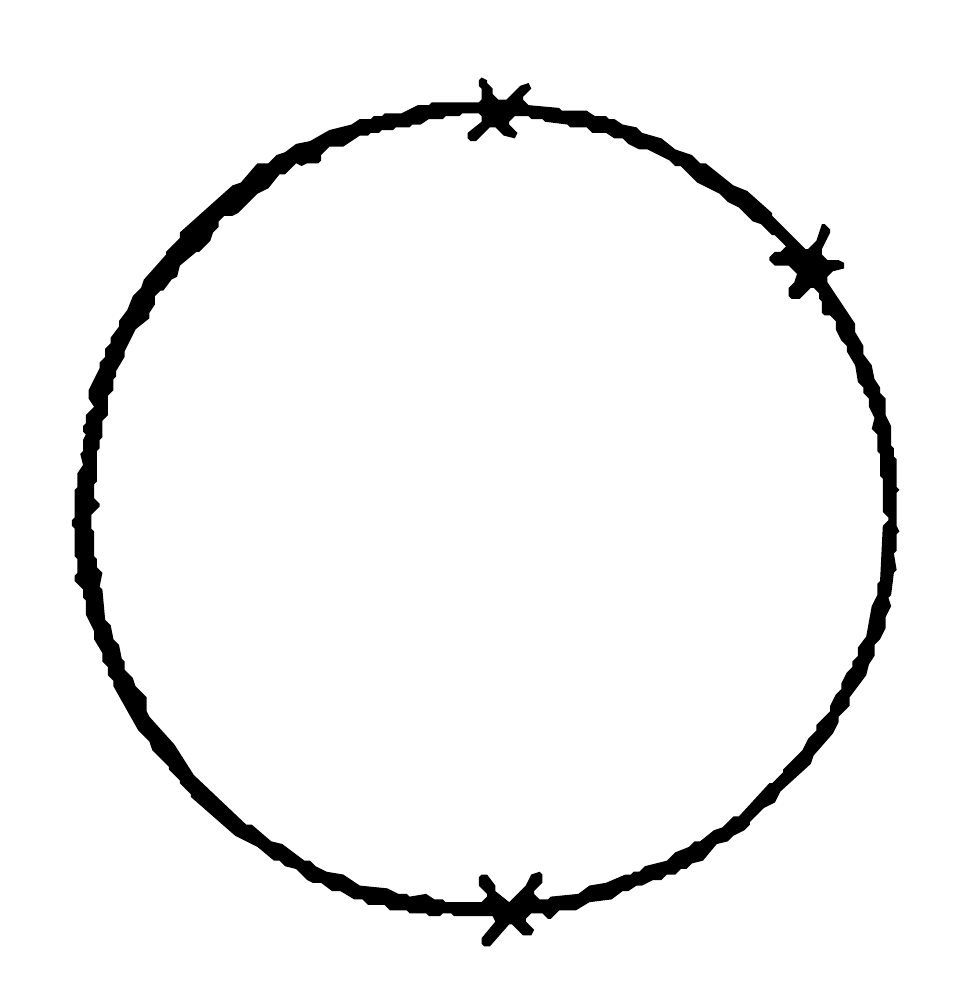
\begin{tikzpicture}[x=1pt,y=-1pt]
\path[use as bounding box] (0,0) rectangle (330,340);
\path[fill=black,draw=none,even odd rule]
(164,18) -- (163,19) -- (163,21) -- (164,22) -- (164,26) -- (163,27) -- (146,27) -- (145,28) -- (141,28) -- (135,31) -- (129,31) -- (128,32) -- (125,32) -- (124,33) -- (120,33) -- (117,35) -- (109,37) -- (102,41) -- (97,42) -- (93,45) -- (90,46) -- (87,49) -- (83,49) -- (77,56) -- (74,57) -- (55,74) -- (55,76) -- (50,81) -- (50,82) -- (42,91) -- (41,94) -- (38,97) -- (36,102) -- (33,106) -- (33,108) -- (30,112) -- (30,114) -- (28,116) -- (28,119) -- (26,121) -- (26,123) -- (22,131) -- (22,134) -- (24,137) -- (21,140) -- (21,143) -- (20,144) -- (20,146) -- (21,147) -- (20,149) -- (20,153) -- (19,154) -- (20,158) -- (18,161) -- (18,166) -- (17,167) -- (17,177) -- (16,178) -- (16,180) -- (17,181) -- (17,191) -- (18,192) -- (18,197) -- (17,198) -- (17,200) -- (20,203) -- (20,206) -- (21,207) -- (21,212) -- (24,218) -- (24,221) -- (27,226) -- (27,229) -- (29,231) -- (29,234) -- (31,236) -- (31,238) -- (40,254) -- (44,258) -- (45,261) -- (51,267) -- (51,268) -- (55,272) -- (55,273) -- (59,277) -- (59,278) -- (75,292) -- (83,296) -- (89,301) -- (91,301) -- (93,303) -- (97,304) -- (101,308) -- (103,309) -- (106,309) -- (110,312) -- (113,312) -- (118,315) -- (121,315) -- (123,317) -- (129,317) -- (131,319) -- (137,319) -- (138,320) -- (144,320) -- (145,321) -- (149,321) -- (150,320) -- (153,320) -- (154,321) -- (168,321) -- (169,323) -- (164,329) -- (164,331) -- (165,332) -- (167,332) -- (174,324) -- (175,324) -- (179,328) -- (182,328) -- (183,326) -- (180,323) -- (180,322) -- (182,320) -- (186,320) -- (188,322) -- (189,322) -- (192,319) -- (198,319) -- (203,316) -- (211,315) -- (215,312) -- (217,312) -- (220,310) -- (222,310) -- (226,308) -- (229,308) -- (231,306) -- (234,306) -- (236,304) -- (238,304) -- (240,302) -- (244,301) -- (249,295) -- (253,294) -- (255,292) -- (259,290) -- (261,288) -- (261,287) -- (266,282) -- (270,280) -- (272,276) -- (283,266) -- (284,263) -- (291,255) -- (293,251) -- (293,249) -- (297,245) -- (297,242) -- (303,234) -- (304,230) -- (306,227) -- (306,223) -- (308,221) -- (310,217) -- (310,213) -- (312,209) -- (311,206) -- (312,205) -- (313,197) -- (314,196) -- (313,190) -- (314,189) -- (314,183) -- (315,182) -- (314,180) -- (314,168) -- (315,167) -- (314,166) -- (314,156) -- (313,155) -- (313,152) -- (312,151) -- (312,144) -- (310,140) -- (310,134) -- (308,132) -- (308,130) -- (306,127) -- (305,122) -- (302,118) -- (302,115) -- (299,110) -- (299,107) -- (289,92) -- (289,90) -- (291,88) -- (295,87) -- (295,85) -- (293,84) -- (289,84) -- (287,82) -- (287,80) -- (290,74) -- (290,73) -- (288,71) -- (287,71) -- (285,77) -- (282,80) -- (281,80) -- (269,68) -- (269,67) -- (260,59) -- (255,57) -- (245,49) -- (243,49) -- (240,46) -- (234,44) -- (229,40) -- (222,38) -- (220,36) -- (215,35) -- (212,33) -- (210,33) -- (209,32) -- (205,32) -- (202,30) -- (193,30) -- (192,29) -- (181,28) -- (179,26) -- (179,25) -- (182,22) -- (181,20) -- (178,21) -- (173,26) -- (170,26) -- (168,24) -- (168,22) -- (166,20) -- (166,19) -- cycle
(157,31) -- (163,31) -- (164,32) -- (164,34) -- (159,38) -- (159,40) -- (160,41) -- (162,41) -- (167,36) -- (169,36) -- (172,39) -- (176,40) -- (177,38) -- (174,35) -- (174,34) -- (176,32) -- (181,32) -- (182,33) -- (186,33) -- (187,34) -- (195,35) -- (196,36) -- (202,36) -- (204,38) -- (209,38) -- (212,40) -- (215,40) -- (217,42) -- (221,44) -- (224,44) -- (232,48) -- (234,50) -- (236,50) -- (242,56) -- (250,60) -- (253,63) -- (257,65) -- (262,70) -- (265,71) -- (269,75) -- (270,75) -- (274,79) -- (272,81) -- (270,81) -- (268,83) -- (268,84) -- (270,86) -- (275,86) -- (278,89) -- (277,92) -- (275,94) -- (275,97) -- (276,98) -- (279,98) -- (283,94) -- (284,94) -- (286,96) -- (286,98) -- (287,99) -- (287,103) -- (288,104) -- (290,104) -- (292,106) -- (292,109) -- (294,113) -- (296,115) -- (296,117) -- (299,122) -- (300,128) -- (302,130) -- (302,132) -- (304,134) -- (304,137) -- (306,141) -- (305,145) -- (307,147) -- (307,153) -- (308,154) -- (308,162) -- (309,163) -- (309,175) -- (311,177) -- (311,178) -- (309,180) -- (308,200) -- (307,201) -- (307,205) -- (305,209) -- (303,220) -- (300,224) -- (300,227) -- (298,229) -- (298,231) -- (296,233) -- (294,237) -- (294,239) -- (292,241) -- (290,245) -- (290,247) -- (285,252) -- (285,254) -- (282,257) -- (280,261) -- (273,268) -- (273,269) -- (269,273) -- (268,273) -- (257,285) -- (255,285) -- (251,289) -- (248,290) -- (243,294) -- (241,294) -- (239,296) -- (234,298) -- (231,301) -- (223,303) -- (221,305) -- (219,305) -- (218,306) -- (216,306) -- (209,309) -- (203,310) -- (199,313) -- (189,314) -- (188,315) -- (185,315) -- (183,313) -- (183,312) -- (186,309) -- (186,306) -- (185,305) -- (182,306) -- (180,310) -- (174,316) -- (169,312) -- (169,310) -- (166,306) -- (164,306) -- (163,307) -- (163,310) -- (166,313) -- (166,314) -- (164,316) -- (151,316) -- (150,315) -- (147,315) -- (144,313) -- (138,314) -- (137,313) -- (134,313) -- (130,311) -- (120,310) -- (114,306) -- (108,305) -- (104,303) -- (102,301) -- (100,301) -- (92,295) -- (88,294) -- (81,288) -- (79,288) -- (60,270) -- (53,259) -- (44,249) -- (43,247) -- (43,242) -- (39,238) -- (38,235) -- (35,232) -- (35,229) -- (34,228) -- (33,223) -- (31,221) -- (30,216) -- (28,214) -- (27,203) -- (26,202) -- (27,197) -- (25,195) -- (25,192) -- (24,191) -- (24,182) -- (23,181) -- (23,176) -- (26,173) -- (26,172) -- (24,170) -- (24,165) -- (25,164) -- (25,153) -- (26,152) -- (26,149) -- (27,148) -- (27,142) -- (29,140) -- (29,133) -- (31,131) -- (31,127) -- (32,126) -- (32,124) -- (35,119) -- (35,117) -- (39,109) -- (44,105) -- (44,103) -- (46,100) -- (46,97) -- (48,95) -- (49,95) -- (52,91) -- (54,90) -- (55,86) -- (61,81) -- (62,81) -- (66,77) -- (67,74) -- (69,72) -- (69,70) -- (71,68) -- (74,68) -- (76,67) -- (83,60) -- (87,58) -- (91,53) -- (93,53) -- (97,49) -- (99,50) -- (101,49) -- (105,49) -- (106,48) -- (106,46) -- (109,43) -- (114,43) -- (120,39) -- (123,39) -- (124,38) -- (127,38) -- (128,37) -- (132,37) -- (133,36) -- (138,36) -- (139,35) -- (142,35) -- (145,33) -- (150,33) -- (151,32) -- (156,32) -- cycle;
\end{tikzpicture}%
}
\end{center}

so ist das Problem unbestimmt.)
\end{minipage}

2) dass sich noch vielerlei zusetzen liesse, wodurch aber anstatt eines Briefes eine Abhandlung entstehen würde, die zu \textls[120]{ordnen} und zu schreiben ich vorerst keine Zeit habe. In der Hoffnung, dass Sie in den Andeutungen vielfachen Stoff zum Nachdenken finden, schliesse ich für heute mit der Bitte mich bald wieder mit einigen Zeilen zu erfreuen.


